\section{Results}
\label{Results}

% \subsection{Defect Density Prediction}
Figures \ref{fig:abn-noc} and \ref{fig:cc-noc} show the distributions of the average bugs number 
(ABN, Fig. \ref{fig:abn-noc}) 
and of clustering coefficient (CC, Fig. \ref{fig:cc-noc}) with respect to the number of communities (NOC) 
for all the sub-projects of all the releases. 
Although the scatterplots for the relationship between NOC % number of communities 
and other metrics are sparse, the reported scatterplots show the existence
of a power-law-like relationship between the maximum values of the mentioned metrics. 
This led us to hypothesize a linear relationship between the maximum values of 
CC and the ABN. % average bug number. If this is the case the CC can be used to predict the maximum ABN % average number of defects 
% in a future release, 
% having cumulated the data belonging to the previous releases.
In Tab. \ref{tab:log-log-cc-noc}, on the left, the power law exponents, 
the correlation coefficient, the $\chi^2$ and the degrees of freedom (\textit{dof}) for the best fitting in log-log scale are reported. 
They refer to different ``cumulated''
releases for the relationship between CC and NOC. % clustering coefficient and the number of communities. 
Table \ref{tab:log-log-cc-noc} shows how the power laws parameters do not change significantly from one cumulated release to another. 
This suggests the existence of a progressively more stable behaviour during 
software evolution, where the fitting with a power law becomes 
more accurate and tends to a fixed value as new releases are added 
in the cumulated dataset.
The same considerations can be applied to the relationship between maximum ABN 
and NOC. % average bugs number and number of communities.
% stabilize around a fixed value
% Namely, with the addition of more releases, .
The scatterplot portraied in Fig. 2 % \ref{cumulated_bug_cc_EC} 
shows the relationship between the maximum defect density versus the maximum clustering coefficient, 
for all the cumulated releases, along with the best fitting straight line.
We investigated if, starting with a dataset of $N$ releases, the best fitting curve for the cumulated $N -1$ releases 
could also be a good fit for the $Nth$ release.
In order to measure the forecast accuracy we adopted a $\chi^2$ test.
Table \ref{tab:max_abn-vs-maxcc} reports the results of the best fitting for the relationship between CC and ABN showing that the linear correlation is not very high. 
Nonetheless, the $\chi^2$ test returns an high level of significance.
Table 2 % \ref{prevision_test} 
reports the results of the analysis on the forecast for software quality. 
We computed the ratio between the $\chi^2$ and the degrees of freedom. 
% The reported $\chi^2$ values are close to 1, meaning that for the given degrees of freedom the fits are good.
According to the results reported on Table \ref{tab:log-log-cc-noc}, on the right, the 
$\chi^2$ values are close to 1, meaning that for the given degrees of 
freedom the fits are good.

\begin{figure*}
        \centering
        \begin{subfigure}%[b]
        {0.3\textwidth}
                \includegraphics[width=\textwidth]{figure/EC_BUG_power_law-eps-converted-to.pdf}
                \caption{Average Bug Number vs. Number of Communities}
                \label{fig:abn-noc}
        \end{subfigure}%
        ~ %add desired spacing between images, e. g. ~, \quad, \qquad, \hfill etc.
          %(or a blank line to force the subfigure onto a new line)
        \begin{subfigure}%[b]
        {0.3\textwidth}
                \includegraphics[width=\textwidth]{figure/EC_CC_power_law-eps-converted-to.pdf}
                \caption{Clustering Coefficient vs. Number of Communities}
                \label{fig:cc-noc}
        \end{subfigure}

        \caption{Scatterplot of the relationships between the studied metrics.}
        \label{fig:scatterplot-abn-cc-noc}
\end{figure*}

\begin{table}%[htbp]
\centering
\begin{tabular}{|c|c|c|c|c|c|}
\hline
\textbf{Releases} & $\alpha$ & $r$ & $\chi^2$ & $dof$  \\
      2.1 - 3-0   & -1.010  & -0.654 &  0.075 & 16 	 \\
      2.1 - 3.1   & - 0.917 & -0.667 &  0.057 & 17 	 \\ 
      2.1 - 3.2   & -0.977  & -0.715 &  0.087 & 20	 \\ 
      2.1 - 3.3   & -0.986  & -0.712 &  0.119 & 21	 \\
\hline
\end{tabular}
\caption{Results on the power law between maximum Clustering Coefficient vs Number of communities for Eclipse: exponent $\alpha$, 
correlation coefficient ($r$), value of Chi Squared ($\chi^2$ ) and number of degrees of freedom ($dof$). 
}
\label{tab:log-log-cc-noc}
\end{table}
\begin{table}
\centering
          \begin{tabular}{|c|c|c|c|c|c|}
	\hline
	\textbf{Eclipse} & max ADD vs NOC & max CC vs NOC \\ 	
		     dof & 13 & 13 \\
		    $\chi^2$ / dof & 0.361 & 1.005 \\ \hline
	      \end{tabular}
\caption{Fit data for the power laws between the maximum average defect density (max ADD) versus the number of communities
and maximum clustering coefficient (max CC) versus the number of communities: correlation coefficient ($r$), 
      normalized Chi squared ($\chi^2$ ), and number of degrees of freedom ($dof$).}
\label{tab:lin-fit-cc-and-add}
\end{table}

\begin{figure*}[!htbp]
     \centering
    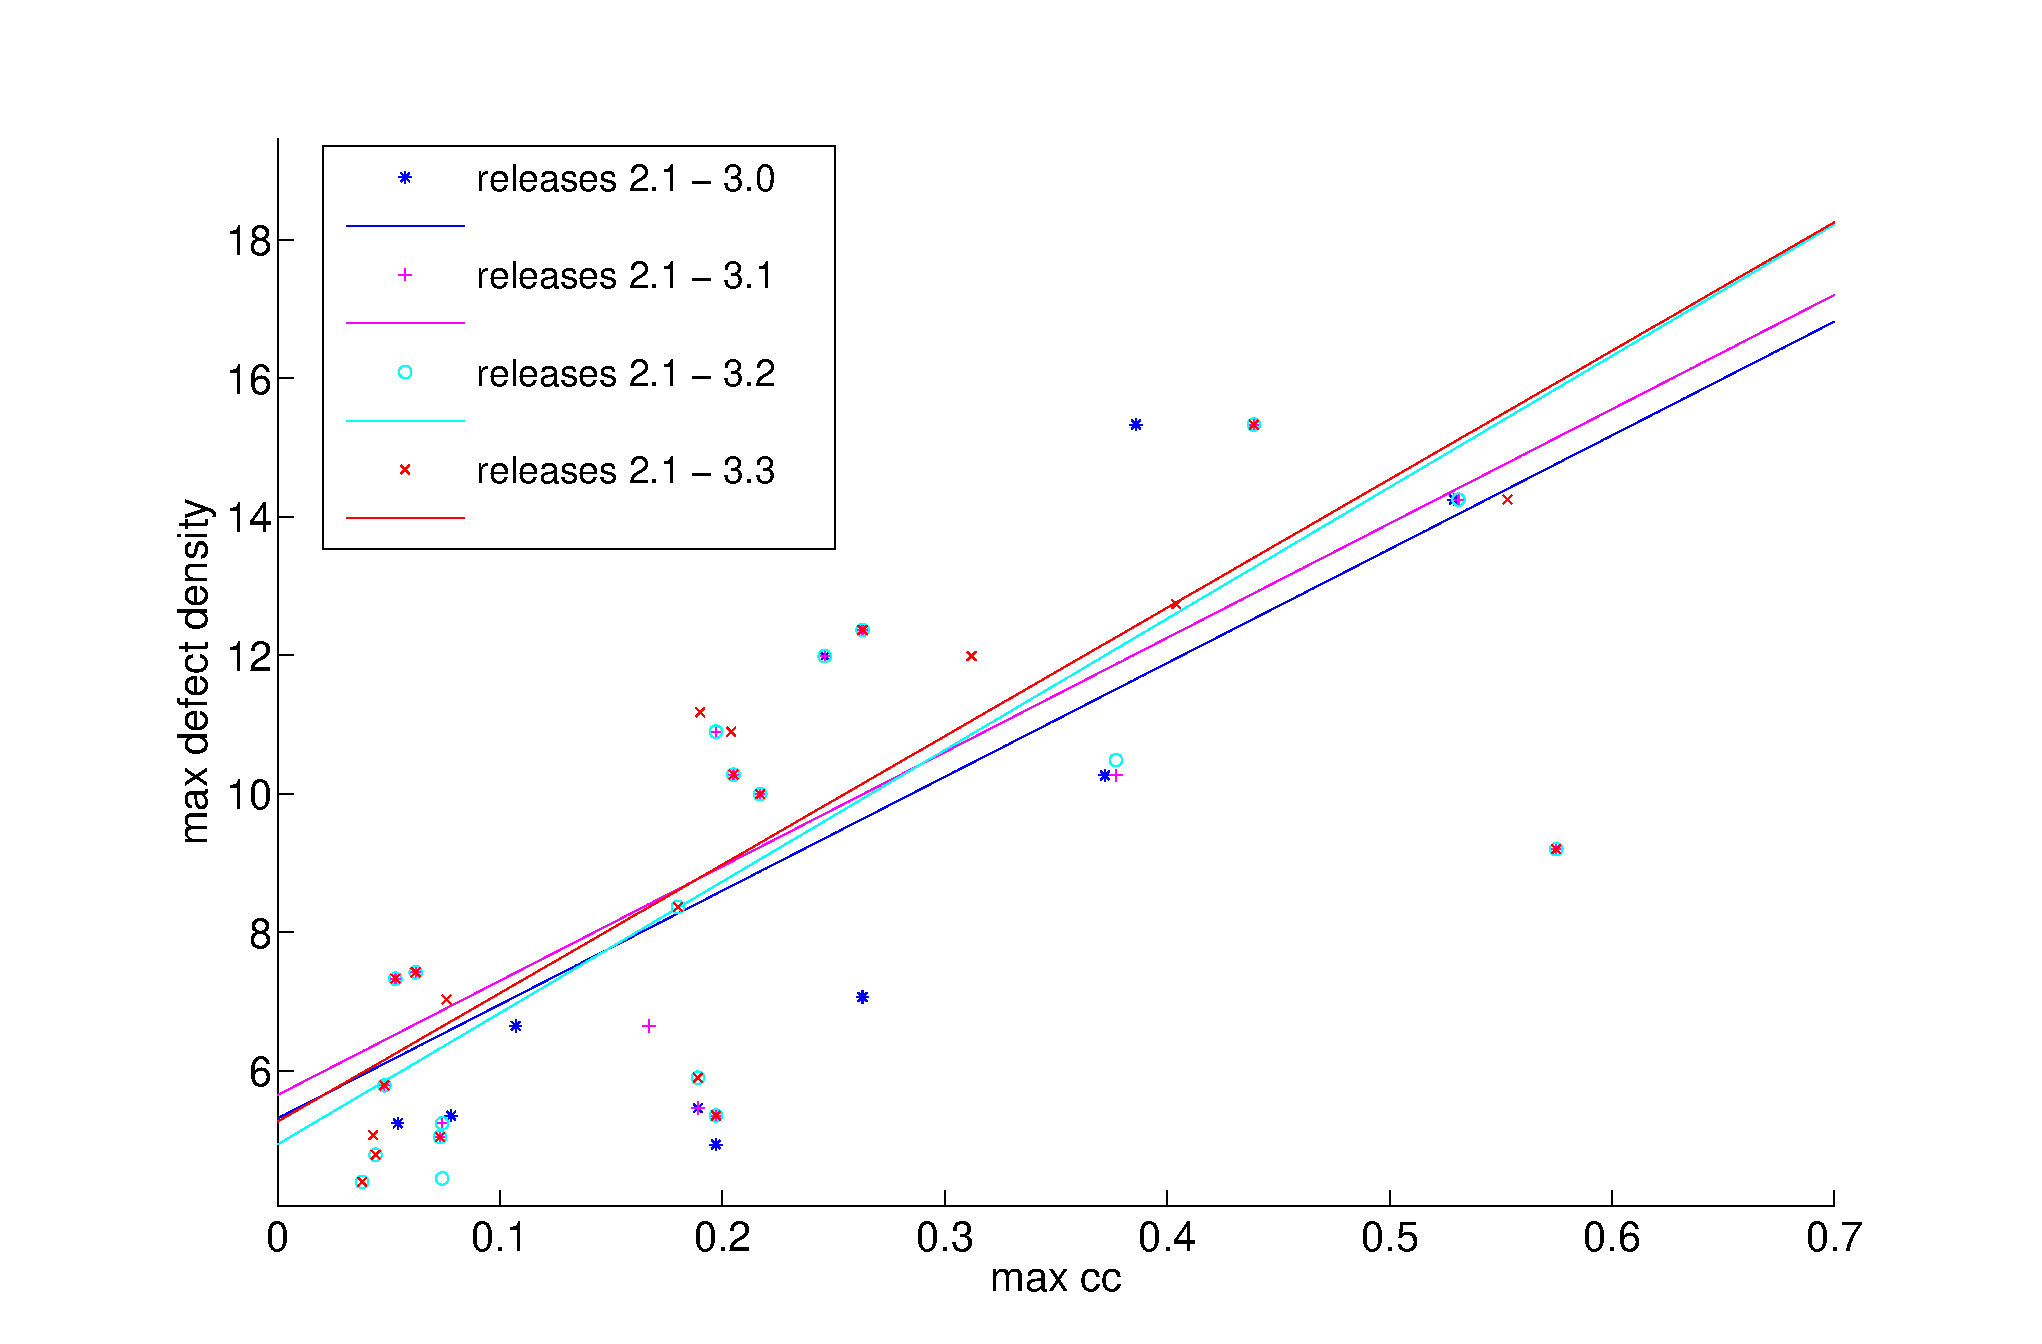
\includegraphics[width=\textwidth]{figure/nuovefig/cumulated_bug_cc_EC.eps}
    \label{cumulated_bug_cc_EC}
    \caption{Cumulated plots and fitting lines for the maximum defect density vs maximum clustering coefficient.}
\end{figure*}

    \begin{table}
    \centering
      \begin{tabular}{|l|c|c|c|}
      \hline
      \textbf{Releases} & $r$ & $\chi^2$ & $dof$  \\
      2.1 - 3-0 & 0.565 & 0.633 & 16  \\
      2.1 - 3.1 & 0.576 & 0.651  & 17  \\
      2.1 - 3.2 & 0.677 & 0.523 & 20 \\ 
      2.1 - 3.3 & 0.687 & 0.547 & 21 \\
      \hline
      \end{tabular}
       \caption{Fit data for the maximum defect density vs maximum clustering coefficient: correlation coefficient ($r$), 
      normalized Chi squared ($\chi^2$ ), and number of degrees of freedom ($dof$).}
\label{tab:max_abn-vs-maxcc}      
\end{table}
  
